\hypertarget{interfaceorg_1_1newdawn_1_1slick_1_1command_1_1_command}{}\section{org.\+newdawn.\+slick.\+command.\+Command Interface Reference}
\label{interfaceorg_1_1newdawn_1_1slick_1_1command_1_1_command}\index{org.\+newdawn.\+slick.\+command.\+Command@{org.\+newdawn.\+slick.\+command.\+Command}}
Inheritance diagram for org.\+newdawn.\+slick.\+command.\+Command\+:\begin{figure}[H]
\begin{center}
\leavevmode
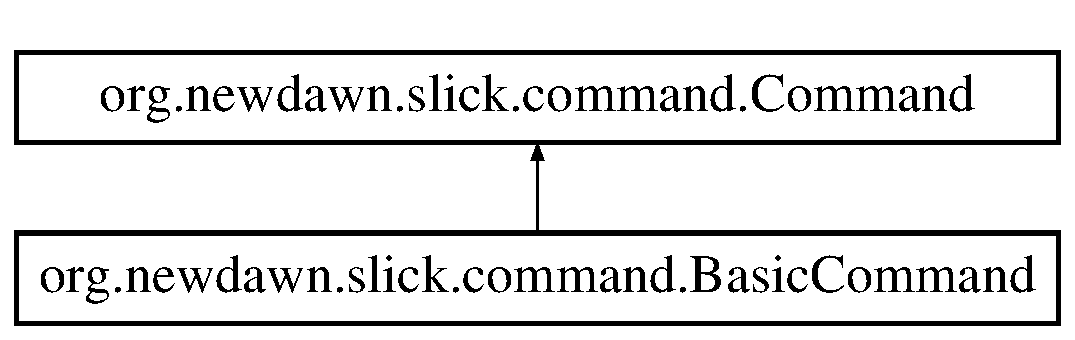
\includegraphics[height=2.000000cm]{interfaceorg_1_1newdawn_1_1slick_1_1command_1_1_command}
\end{center}
\end{figure}


\subsection{Detailed Description}
The description of a action feedback from the abstract input system. This marker allows the creation of action objects that can contain useful state. If you don\textquotesingle{}t need state and just a name use {\ttfamily \mbox{\hyperlink{classorg_1_1newdawn_1_1slick_1_1command_1_1_basic_command}{Basic\+Command}}$<$/code.}

{\ttfamily \begin{DoxyAuthor}{Author}
kevin 
\end{DoxyAuthor}
}